% Options for packages loaded elsewhere
\PassOptionsToPackage{unicode}{hyperref}
\PassOptionsToPackage{hyphens}{url}
\documentclass[
  ignorenonframetext,
]{beamer}
\newif\ifbibliography
\usepackage{pgfpages}
\setbeamertemplate{caption}[numbered]
\setbeamertemplate{caption label separator}{: }
\setbeamercolor{caption name}{fg=normal text.fg}
\beamertemplatenavigationsymbolsempty
% remove section numbering
\setbeamertemplate{part page}{
  \centering
  \begin{beamercolorbox}[sep=16pt,center]{part title}
    \usebeamerfont{part title}\insertpart\par
  \end{beamercolorbox}
}
\setbeamertemplate{section page}{
  \centering
  \begin{beamercolorbox}[sep=12pt,center]{section title}
    \usebeamerfont{section title}\insertsection\par
  \end{beamercolorbox}
}
\setbeamertemplate{subsection page}{
  \centering
  \begin{beamercolorbox}[sep=8pt,center]{subsection title}
    \usebeamerfont{subsection title}\insertsubsection\par
  \end{beamercolorbox}
}
% Prevent slide breaks in the middle of a paragraph
\widowpenalties 1 10000
\raggedbottom
\AtBeginPart{
  \frame{\partpage}
}
\AtBeginSection{
  \ifbibliography
  \else
    \frame{\sectionpage}
  \fi
}
\AtBeginSubsection{
  \frame{\subsectionpage}
}
\usepackage{iftex}
\ifPDFTeX
  \usepackage[T1]{fontenc}
  \usepackage[utf8]{inputenc}
  \usepackage{textcomp} % provide euro and other symbols
\else % if luatex or xetex
  \usepackage{unicode-math} % this also loads fontspec
  \defaultfontfeatures{Scale=MatchLowercase}
  \defaultfontfeatures[\rmfamily]{Ligatures=TeX,Scale=1}
\fi
\usepackage{lmodern}
\ifPDFTeX\else
  % xetex/luatex font selection
\fi
% Use upquote if available, for straight quotes in verbatim environments
\IfFileExists{upquote.sty}{\usepackage{upquote}}{}
\IfFileExists{microtype.sty}{% use microtype if available
  \usepackage[]{microtype}
  \UseMicrotypeSet[protrusion]{basicmath} % disable protrusion for tt fonts
}{}
\makeatletter
\@ifundefined{KOMAClassName}{% if non-KOMA class
  \IfFileExists{parskip.sty}{%
    \usepackage{parskip}
  }{% else
    \setlength{\parindent}{0pt}
    \setlength{\parskip}{6pt plus 2pt minus 1pt}}
}{% if KOMA class
  \KOMAoptions{parskip=half}}
\makeatother
\usepackage{graphicx}
\makeatletter
\newsavebox\pandoc@box
\newcommand*\pandocbounded[1]{% scales image to fit in text height/width
  \sbox\pandoc@box{#1}%
  \Gscale@div\@tempa{\textheight}{\dimexpr\ht\pandoc@box+\dp\pandoc@box\relax}%
  \Gscale@div\@tempb{\linewidth}{\wd\pandoc@box}%
  \ifdim\@tempb\p@<\@tempa\p@\let\@tempa\@tempb\fi% select the smaller of both
  \ifdim\@tempa\p@<\p@\scalebox{\@tempa}{\usebox\pandoc@box}%
  \else\usebox{\pandoc@box}%
  \fi%
}
% Set default figure placement to htbp
\def\fps@figure{htbp}
\makeatother
\setlength{\emergencystretch}{3em} % prevent overfull lines
\providecommand{\tightlist}{%
  \setlength{\itemsep}{0pt}\setlength{\parskip}{0pt}}
\usepackage{bookmark}
\IfFileExists{xurl.sty}{\usepackage{xurl}}{} % add URL line breaks if available
\urlstyle{same}
\hypersetup{
  hidelinks,
  pdfcreator={LaTeX via pandoc}}

\author{\texorpdfstring{}{}}
\date{}

\begin{document}

\begin{frame}{The 1816 Coinage Act as Topological Regression}
\protect\phantomsection\label{sec-coinage-act-1816}
While Blake proposed a visionary resolution to the meta-stable friction
of Twofold Generation through infinite, Fourfold spiritual expansion,
the British state pursued the exact opposite trajectory. Reacting
against both the swerve of unbacked paper money (see
\hyperlink{sec-bank-restriction-1797}{§ The 1797 Bank Restriction}) and
the arbitrage of the bullion trade, the government sought a rigid
anchor.

\begin{block}{Lord Liverpool's Act: The Legislative Architecture of
Monometallism}
\protect\phantomsection\label{lord-liverpools-act-the-legislative-architecture-of-monometallism}
Under the guidance of Lord Liverpool, Parliament passed the Coinage Act
of 1816 (56 Geo. III c.68) on \textbf{22 June 1816}, officially known as
``An Act to provide for a New Silver Coinage, and to regulate the
Currency of the Gold and Silver Coin of this Realm.'' This Act legally
demonetized full-bodied silver entirely as a standard of value. It
relegated silver to a mere token coinage---reduced in weight to 66
shillings per troy pound from the prior 62 shillings, and declared legal
tender only for amounts up to \textbf{40 shillings}---effectively ending
the bimetallic alchemical marriage of the previous centuries and
enforcing a strict \emph{de jure} Gold Standard
{[}@redish1990evolution{]}. The new gold sovereign was defined at
\textbf{123.274 grains} (7.988 grams) of standard \textbf{22-carat gold}
(91.67\% pure), with one troy pound of standard gold equivalent to
\textbf{£46 14s 6d} (44½ guineas). This sovereign coin would become the
foundation of British imperial finance for a century.
\end{block}

\begin{block}{The Mathematical and Thermodynamic Necessity of Bimetallic
Collapse}
\protect\phantomsection\label{the-mathematical-and-thermodynamic-necessity-of-bimetallic-collapse}
The mathematical necessity of this collapse is formalized by Velde's
border conditions for bimetallism. For both metals to circulate
concurrently, the global commodity price ratio (\(P_G^G / P_G^S\)) must
dynamically satisfy strict world monetary demand shares (\(m_G, m_S\)):

\begin{equation}
\label{eq:velde_demand_shares}
m_G (1 - m_G) < \frac{P_G^G}{P_G^S} < \frac{(1 - m_S)}{m_S}
\end{equation}

By legally tokenizing silver (\(m_S \to 0\) as a standard of sovereign
reserve), the 1816 Coinage Act intentionally violated this inequality,
mathematically engineering a permanent structural singularity
{[}@velde2005bimetallism; @quinn1996competing{]}. Lord Liverpool and the
architects of the Act did not ``resolve'' the crisis of human value;
rather, from a Blakean perspective, they triggered a topological
regression back into the quantification of \textbf{Single Vision
(Ulro)}.
\end{block}

\begin{block}{The Chimeric Regime and the Amputation of Silver}
\protect\phantomsection\label{the-chimeric-regime-and-the-amputation-of-silver}
As Joseph Albernaz theorizes in his work on common wealth, totalizing
measurement regimes like the Gold Standard operate as deeply
``chimeric'' technologies. They enforce false ontologies to ``ground'' a
community, purposefully obfuscating humanity's shared
``groundlessness''---our fundamental interdependence
{[}@albernaz2024common{]}. The 1816 Act was the finalized Urizenic
framing of the British economy. The structural bimetallic tension
(Twofold Vision) was erased not by synthesizing gold and silver into a
higher qualitative order of human flourishing, but by amputating the
lunar element of silver entirely. By tying the productive capacity of
the British Empire to one isolated, calculable element---the 22-carat
sovereign---the state surrendered to the condition where nothing exists
unless it can be mathematically derived from gold. The social
consequences were severe: as Del Mar documents, the contraction of the
monetary base that followed silver's demonetization enriched the
creditor class while plunging the producing classes into deflationary
poverty---a transfer of wealth from labor to capital that Blake's
\emph{Jerusalem} had prophetically condemned as the ``curb / Of Poverty
on the laborious'' {[}@delmar1895history; @erdman1988complete{]}.

Blake renders this financial taming of living energy with characteristic
precision on Plate 55 of \emph{Jerusalem}, where the nations of empire
appear as wild forces subjugated by monetary instruments:

\begin{quote}
``Curbing their Tygers with golden bits \& bridles of silver \& ivory.''
(\emph{Jerusalem}, Plate 55; Erdman p.~205) {[}@erdman1988complete{]}
\end{quote}

The image is economically exact: empire tames its subject peoples not
with violence alone but with the golden bits (gold standard coercion)
and silver bridles (the compliant token coinage of the colonies) that
enforce subordination. The ``ivory''---a colonial commodity extracted
from Africa---completes the triad of imperial extraction. Gold bits,
silver bridles: the exact instruments of the bimetallic system (gold
standard with silver relegated to token status under the 1816 Act)
deployed as tools of subjugation. Blake's vision extends beyond British
monetary policy to the global architecture of imperial finance: the 1816
Act did not merely tokenize silver domestically---it exported the
Urizenic framework to every territory the Empire controlled, binding
colonial economies to the gold sovereign and severing them from their
own internal bimetallic circulations.

\begin{figure}
\centering
\pandocbounded{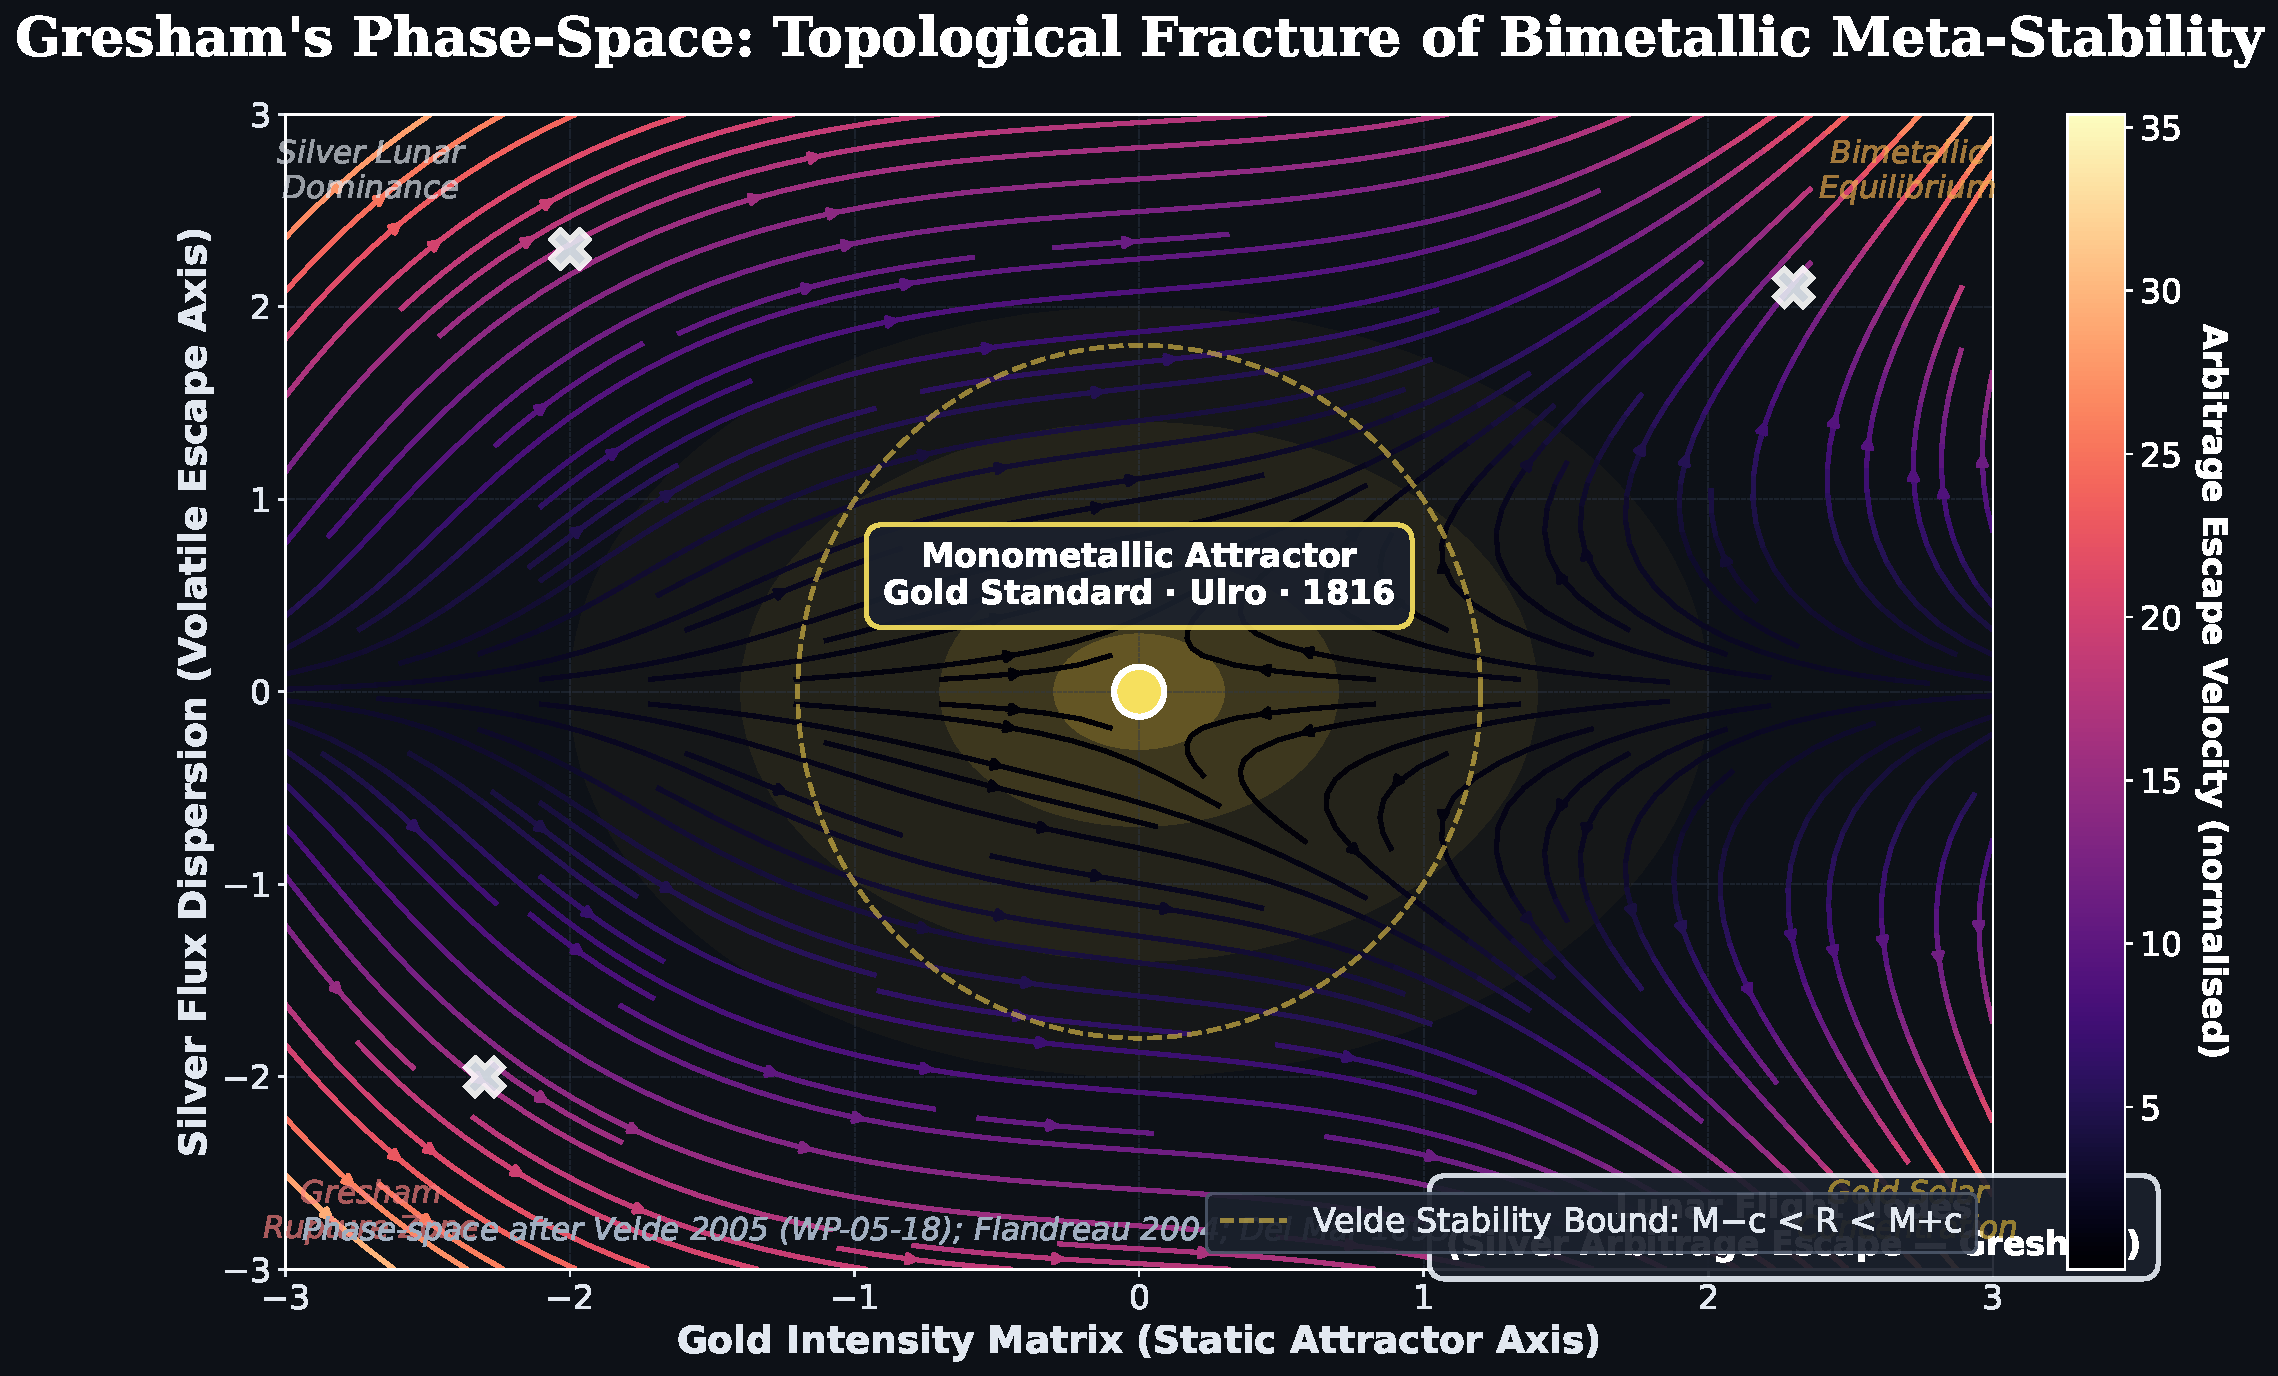
\includegraphics[keepaspectratio,alt={Topological Fracture of Gresham's Law in Phase-Space. This dynamic magma streamplot on a 120×120 grid visualizes the macroeconomic collapse of bimetallic metastability. An overlaid dashed golden ellipse denotes the Velde stability boundary M - c \textless{} R \textless{} M + c. The geometric center (Gold Attractor, m\_S \textbackslash to 0 / Ulro / 1816 Singularity, rendered with a four-layer glow ring) exerts an inflexible inward-pulling vector field (U = -X + 2Y\^{}2)---the gravitational well of the monometallic standard: the 22-carat sovereign at 123.274 grains freezing human exchange into static atoms of sovereign credit. The outward thermal-gradient vectors represent the Lunar Flight (V = 0.5Y + YX\^{}2): silver arbitrage shattering its state-mandated bond into three distinct silver flight nodes (marker `X'). As the Mint Ratio (M) diverges structurally from the international Market Ratio (R), the currency system undergoes topological clinamen out of the bimetallic equilibrium quadrant into the Gresham rupture zone. The 1816 Coinage Act enforced the terminal Urizenic amputation of silver, restricting token coinage to 40 shillings.}]{../figures/topological_fracture_dark.pdf}}
\caption{Topological Fracture of Gresham's Law in Phase-Space. This
dynamic magma streamplot on a 120×120 grid visualizes the macroeconomic
collapse of bimetallic metastability. An overlaid dashed golden ellipse
denotes the Velde stability boundary \(M - c < R < M + c\). The
geometric center (Gold Attractor, \(m_S \to 0\) / Ulro / 1816
Singularity, rendered with a four-layer glow ring) exerts an inflexible
inward-pulling vector field (\(U = -X + 2Y^2\))---the gravitational well
of the monometallic standard: the 22-carat sovereign at 123.274 grains
freezing human exchange into static atoms of sovereign credit. The
outward thermal-gradient vectors represent the Lunar Flight
(\(V = 0.5Y + YX^2\)): silver arbitrage shattering its state-mandated
bond into three distinct silver flight nodes (marker `X'). As the Mint
Ratio (\(M\)) diverges structurally from the international Market Ratio
(\(R\)), the currency system undergoes topological clinamen out of the
bimetallic equilibrium quadrant into the Gresham rupture zone. The 1816
Coinage Act enforced the terminal Urizenic amputation of silver,
restricting token coinage to 40 shillings.}\label{fig-topology}
\end{figure}
\end{block}

\begin{block}{The Victory of ``Single Vision \& Newton's Sleep''}
\protect\phantomsection\label{the-victory-of-single-vision-newtons-sleep}
This systemic reduction was the ultimate victory of ``Single vision \&
Newtons sleep'' (as Blake declared in his 1802 letter to Butts; Erdman
p.~720) {[}@erdman1988complete{]}. It represented a reduction of the
regenerate 4-fold man back into an isolated, atomized economic cog,
evaluated solely against the geometric weight of the new golden
sovereign coin. It was a regression into intellectual and spiritual
infancy under the guise of scientific finance, establishing a paradigm
of scarcity that Blake would fight until his last breath. The arc from
Newton's 1717 ratio through the 1797 Restriction to the 1816 Act traces
a complete Blakean narrative: from the imposition of Urizenic geometry
upon the living economy, through the chaotic void of paper abstraction,
to the final re-assertion of monometallic control. Blake's prophetic
response---the immense, unfinished architecture of \emph{Jerusalem},
composed across exactly these years---constitutes the most sustained
imaginative resistance to this economic ontology in the entire literary
canon.
\end{block}
\end{frame}

\end{document}
